% Created 2017-06-07 Wed 21:33
% Intended LaTeX compiler: pdflatex
\documentclass[12pt]{article}
\usepackage[utf8]{inputenc}
\usepackage[T1]{fontenc}
\usepackage{graphicx}
\usepackage{grffile}
\usepackage{longtable}
\usepackage{wrapfig}
\usepackage{rotating}
\usepackage[normalem]{ulem}
\usepackage{amsmath}
\usepackage{textcomp}
\usepackage{amssymb}
\usepackage{capt-of}
\usepackage[colorlinks=true]{hyperref}
\usepackage{minted}
\usepackage[usenames,dvipsnames]{xcolor}
\usepackage{braket}
\usepackage[margin=1.0in]{geometry}

%% \usepackage[
%%   activate={true,nocompatibility},
%%   final,
%%   kerning=true
%% ]{microtype}

\usepackage[
  inline = true,
  margin = false,
  status = draft,
]{fixme}
\fxusetheme{color}

\usepackage[
    backend     = biber,
    style       = chem-acs,
    autocite    = superscript,
    doi         = true,
    maxbibnames = 1000,
]{biblatex}
\setlength\bibitemsep{0pt}
\renewcommand*{\bibfont}{\footnotesize}
\let\cite\autocite

\addbibresource{./assignment7.bib}

\author{Eric Berquist}
\date{June 15th, 2017}
\title{Deciphering the Contents of Chemically-Trained Neural Networks into Physical Intuition}
\hypersetup{
 pdfauthor={Eric Berquist},
 pdftitle={Deciphering the Contents of Chemically-Trained Neural Networks into Physical Intuition},
 pdfkeywords={},
 pdfsubject={},
 pdfcreator={Emacs 25.2.1 (Org mode 9.0.8)}, 
 pdflang={English}, 
 colorlinks=true, 
 linkcolor=MidnightBlue, 
 citecolor=MidnightBlue, 
 urlcolor=MidnightBlue}
\begin{document}

\maketitle

\section{Overview and Objectives}
\label{sec:org1773cf1}

The explosive growth of computing power has enabled the use of machine learning (ML) models for the accurate calculation of chemical properties. Current ML models are capable predicting energetic properties of small, neutral organic molecules to chemical accuracy (1 kcal/mol)\cite{2017arXiv170205532F}. However, it is unclear \emph{what} the quality of a prediction will be when a ML model is given a molecule outside its training set, and \emph{why} the model is giving that prediction. Each ML model is a set of unknown parameters that constitute a black box \cite{wiki:blackbox}, where it is not known or understood \emph{how} the model functions, \emph{why} the model gives the predictions it does, and \uline{whether or not correct predictions are being made for the right reasons}\cite{2017arXiv170303717S}. A critical step for the continued application of ML models to quantum chemistry will be to make predictions beyond the relatively simple example systems that are currently seeing widspread use \cite{Ramakrishnan:2014ij}. Some of the most important, interesting, and unexplored chemistry in terms of reactivity and intrinsic molecular properties involves species that are either charged or have unpaired electrons, both of which are outside the scope of current applications. If a model is not right for the right reasons, there cannot be an expectation that it is transferable to even similar inputs, and is an indicator that the architecture is insufficient for training on more complex datasets. Such a battle is being fought within electronic structure theory\cite{Zhao2008,Medvedev49,Kepp496,Medvedev496}, with the most negative potential consequence being invalidation of the past decade's application of quantum chemical methods to chemical problems.

The \uline{overall objective} is to quantify what quantum chemistry-trained machine learning models are actually learning. The \uline{central hypothesis} is that the application of machine learning to quantum chemistry is physically motivated, \emph{i.e.}, ML models are learning parameters that connect the molecular representation (input features) to predictions in a manner that is qualitatively identical to how a trained chemist would apply their intuition. An implicit connection has already been made \cite{2017arXiv170205532F} between how a molecule is represented as input to ML models and the accuracy of prediction for certain kinds of properties, but this connection has not been explored. The \uline{rationale} is that by understanding the connection between the molecular representation given to ML models and their predictions, ML models themselves can be used for rationalizing molecular structure-property relationships. The overall objective will be achieved through the following \uline{specific aims}:

\begin{enumerate}
\item \textbf{Reproduce existing machine learning models for molecular properties from the literature.} I will replicate two neural networks (NNs) from \parencite{2017arXiv170205532F} to serve as both the necessary architecture that analysis tools developed later in this proposal will be built on, and as the baseline for prediction accuracy. NNs are chosen since they overall exhibit the most quantitatively accurate predictions compared to other ML architectures when trained on quantum chemical data. I will reproduce the isotropic static polarizability \(\bar{\alpha}\) \parencite{POC:POC407} and the zero-point vibrational energy \(E_\text{ZPVE}\) \parencite{doi:10.1063/1.2436891}, which represent molecular properties that can be derived from spectroscopic observables and are difficult to predict with current NN approaches.

\item \textbf{Characterize the parameters learned by existing machine learning models from the literature.} I will use relevance propagation \cite{10.1371/journal.pone.0130140,Binder2016,JMLR:v17:15-618} to quantify the relative importance of each input feature for each predicted property of the NNs in aim \#1. Relevance propagation gives insight into a model's learned coefficients in a fashion that can be used directly in statistical analysis and visualization.

\item \textbf{Train supervised neural networks on complex molecular properties.} Using the molecular database from aim \#1, I will predict their vibrational and nonlinear optical properties, specifically the static parallel first hyperpolarizability \(\beta_{\parallel}\) \parencite{doi:10.1063/1.3134744} and the set of frequencies \(\{\tilde{\nu}\}\) that compose stick vibrational spectra, as they represent a natural extension in complexity from \(\bar{\alpha}\) and \(E_{\text{ZPVE}}\).

\item \textbf{Characterize the parameters learned for complex molecular properties using unsupervised neural networks.} I will use the relevance propagation techniques developed in aim \#2 to show the underlying causes for the performance of the NNs trained in aim \#3. To aid in quantifying the importance of molecular features to property predictions, I will train a denoising autoencoder-based neural network in an unsupervised manner to provide a compressed representation of molecular inputs. Unsupervised NNs are capable of discovering intrinsic properties of their input samples \cite{VincentPLarochelleH2008}, which will provide a summarized interpretation of molecular structure importance when combined with relevance propagation.
\end{enumerate}

The \uline{expected outcomes} are

\begin{itemize}
\item clear connections between the input molecular representations and predicted outputs that can be used to build quantitative structure-function relationships, that
\item adding an unsupervised learning stage provides a reduced-dimensionality molecular representation connecting directly to chemical intuition,
\item well-defined and publicly-available protocols for applying more complex ML models to chemical properties, regarding all stages of the prediction pipeline: generation of the QM data from calculations, preparation of the input, training of the model, and analysis of the results, and
\item ML models capable of predicting complex molecular properties, with the first proof-of-concept predictions of higher-order nonlinear optical properties and vibrational spectra.
\end{itemize}

\section{Significance}
\label{sec:orgf8bad22}

This is the first attempt at understanding the parameters of ML models used to predict microscopic and macroscopic molecular properties, rather than treating the models as black boxes that cannot be understood. If ML models are shown to be learning physically-motivated or chemically-intuitive parameters, ML can become more than just a path for the accurate prediction of molecular properties, but be transformed into a tool itself that can give deep insight into molecular structure-property relationships. ML models are expensive to train, maintain, and extend in terms of both human and CPU time\cite{43146}. If this proposal shows that ML models are not learning properly, then the scientific research community can avoid the wasteful use of resources on model training and shift their focus to developing better model architectures than the current state-of-the-art.

\section{Review of Relevant Literature}
\label{sec:orge06502d}

\subsection{Machine Learning}
\label{sec:orgb6ea6b8}

Machine learning is the ability for computers to ``learn'' without being given explicit instructions. Rather than providing exact instructions though traditional programming, computers are fed sets of input data and are usually expected to return a certain result. By training itself to reproduce results, a learned ML model would ideally be able to predict outputs for new, unknown inputs. Common applications of ML are in email spam filtering, search engine prediction, image and voice recognition, and self-driving cars.

Some definitions and terms used throughout this proposal are

\begin{itemize}
\item \emph{Architecture}: the formal structure of the network or ML model itself, encompassing the region from equations and diagrams to the implementation (code).
\item \emph{Model}: an architecture implemented in code with learned parameters.
\item \emph{Pipeline}: multiple steps and components chained together, such as the preparation of data for input into an architecture, the architecture itself, and any steps required to transform the architecture output into something else useful, such as visualizations or statistics.
\end{itemize}

The two types of learning used in this proposal are

\begin{itemize}
\item \emph{Supervised learning}: Train a machine learning model using data where the correct output prediction is known and given for each input sample, and the goal of the model is to predict similar types of outputs for new inputs.
\item \emph{Unsupervised learning}: Train a machine learning model using data where the correct output prediction is not given, and the goal of the model is to learn intrinsic properties of the inputs by recreating the input as output.
\end{itemize}

\subsection{Machine Learning in Chemistry}
\label{sec:orga0bc40b}

The use of machine learning to make chemical predictions is not new, with work dating back over 25 years for prediction of NMR spectra using small neural networks trained on experimental data \cite{THOMSEN1989212}. The largest application of machine learning to chemical problems is within cheminformatics, where it has seen wide use within industrial drug discovery with emphasis on predicting quantitative structure-activity relationships (QSAR) \cite{doi:10.1080/17460441.2016.1201262}. The goal is to predict the activity of a given drug candidate based on experimental activities of many other molecules, with inputs being information about atom types, bond types, number of aromatic rings, atomic partial charges, and other pieces of structural information, all of which are related to the molecular graph or connectivity \cite{Kearnes2016}.

In particular, there is a recent application of deep neural networks (DNNs) to QSAR datasets\cite{doi:10.1021/ci500747n}, which contains a systematic study for determining the best model parameters. The machine learning community calls this ``hyperparameter tuning'', which is another term for parameter optimization. However, this is still an empirical black-box approach, where the input is manually manipulated and statistical analysis is performed on the output, but this does not provide enough insight into how or why the quality of a model changes. For example, whether or not a rectified linear unit (ReLU) or sigmoid unit is the best function to represent neuron activation says nothing about why one molecule may be more potent than another in a QSAR study. This brute-force type of parameter optimization \emph{does} provide a good starting point for understanding the sensitivity of a ML model. Unfortunately, even parameter optimization has not been extensively performed on models trained using quantum chemical data. In that sense, cheminformatics is a step ahead of other sub-disciplines in chemistry regarding the \emph{application} of machine learning models, but not in the \emph{understanding} of their models. 

Their parameter optimization study is especially relevant to this proposal because it examines the effect of placing an unsupervised NN before other NNs for unsupervised pretraining. Surprisingly, the authors found that an unsupervised pretraining step decreased the accuracy of their predictions, which is counter to the expected outcome of this proposal. However, the paper implies that their results are not even valid due to algorithmic restrictions in their software. Therefore it seems incorrect to draw any conclusions from this, such as ``no unsupervised pretraining is needed''. It would be interesting to see if the same conclusion is drawn for models trained on quantum chemical data using the proper algorithms.

Additionally, it is unclear why a DNN trained on the combination of all QSAR datasets (called a ``joint DNN'') performs better than separate DNNs for each dataset when considering the lack of overlap in the training sets. The methods developed in this proposal, while being applied to models trained on quantum chemical data, should be applicable to any DNN (consider that relevance propagation is mostly developed in computer vision/image recognition). One goal of this proposal is to transfer the idea of relevance propagation from its original intended application field to other fields. If it is indeed transferable, then it may shed some light on why unsupervised learning resulted in decreased prediction performance and the improvement of join DNNs over separate DNNs.

\subsection{Machine Learning in Quantum Chemistry}
\label{sec:org6ed44c3}

However, the use of machine learning in quantum chemistry, specifically electronic structure theory, is relatively new, with the earliest references on Scopus dating back to 2008, a large spike in 2013, and rapid growth from 2015 to today. The goal is to predict more elemental properties than within cheminformatics, such as the internal energy, enthalpy, free energy, heat capacity, HOMO and LUMO energies and gaps, dipole moments, polarizabilities, and zero-point vibrational energies\cite{2015arXiv150204563R}. More advanced applications are the use of neural networks for predicting the products of organic reactions\cite{doi:10.1021/acscentsci.6b00219} and the transport properties of candidates for organic photovoltaics\cite{C5SC04786B}.

There have not been attempts to predict tensorial properties, just scalar-valued properties. This precludes the prediction of full spectroscopic properties, which are mathematically not representable as single scalars. There is recent work considering the prediction of full spectra, specifically linear vibrational spectra from \emph{ab initio} molecular dynamics (AIMD) simulations\cite{2017arXiv170505907G}. However, this proposal is concerned with the generation of spectra from static calculations, which avoids some convolution of the calculated spectra being dependent on the model's learned representation of the potential energy surface. Additionally, their vibrational spectra were calculated from the dipole autocorrelation function, which is dependent on artificially partitioning the electron density into atomic charges, which they derive from the neural network. Thus, this is not an end-to-end \cite{2016arXiv160407316B} prediction of molecular spectra from a single structure, as will be performed in this proposal. By performing end-to-end prediction rather than decomposing the problem so that the neural network only considers part of the prediction task, this proposal pushes the limits of attempting to train neural networks on the prediction of complex molecular properties.

\subsection{Relevance Propagation}
\label{sec:org28d36fa}

Layer-wise relevance propagation (LRP, or relevance propagation) is a method for identifying what a ML model has learned \cite{10.1371/journal.pone.0130140} in terms of the model's input features. Figure \ref{fig:org7673d07} is a concrete example of what the output from relevance propagation looks like when applied to image classification by a neural network. Here, we assume that the network correctly identified the subject of the image as a cat (rather than a dog or a potted plant), but relevance propagation shows which image pixels were most important for the network to determine the photo is of a cat. The pixel-wise importance is a single number for each pixel that can be interpreted as a contribution for that pixel to the final classification of the image. More generally, is it the relative importance of each input feature to the predicted output; here and in other image recognition examples, pixels are input features. Applications to image classification resulting in pixel importance naturally lends itself to visualizing the output as a heatmap on top of the original input.

\begin{figure}[htbp]
\centering
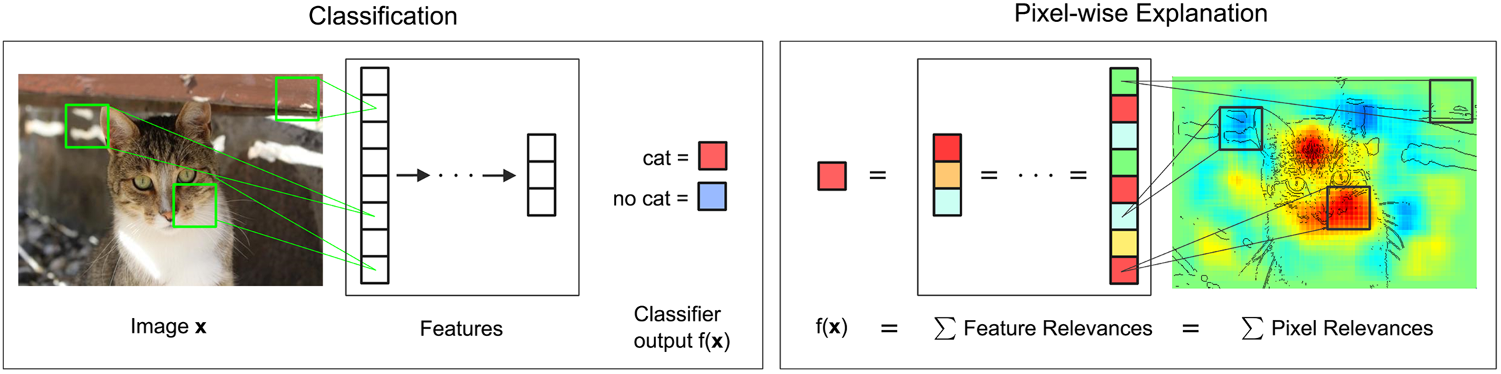
\includegraphics[width=.9\linewidth]{2-Figure1-1.png}
\caption{\label{fig:org7673d07}
Example of output from relevance propagation showing which sections of an image the neural network considered important during classification. Taken from \parencite{10.1371/journal.pone.0130140}.}
\end{figure}

Other methods exist for assigning rules of how input features map to predictions \cite{Finnegan105957,2017arXiv170303717S,2016arXiv161107478L}. Several of these are based on the idea of gradient perturbations, where repeated changes in prediction are measured as a result of small changes in the input. Performed enough times, this creates a map of the network's decision boundary\cite{wiki:db}. A gradient perturbation-based method is unsatisfactory because it requires repeated forward passes through the network with a set value for the perturbation size, and relevance propagation requires only one backward pass with a single free but insensitive parameter. Additionally, most methods for assigning input relevance have only been used for image classification, where the input features are of uniform type (pixel data). The input featurization for representing molecular structures\cite{2017arXiv170205532F} is heterogeneous, and it is unclear how the perturbation parameter should be varied for each kind of molecular feature.

The closest use of input relevance in molecular predictions is monitoring the evolution of input features as network training progresses\cite{Kearnes2016}, shown in \ref{fig:orga0957c9}. However, there is no definition for what the evolution of input features is, such as the metric for evolution, or what the units are. One aim of this proposal is to form a quantitative basis connecting molecular features to model predictions that figures such as \ref{fig:orga0957c9} can be built upon.

Although no improvements will be made to the basic relevance propagation algorithm itself, there is novelty in two areas. To the best of the PI's knowledge, this is the first time relevance propagation will be applied to a regression task rather than a classification task, and the first time relevance propagation will be applied outside of image classification.

\begin{figure}[htbp]
\centering
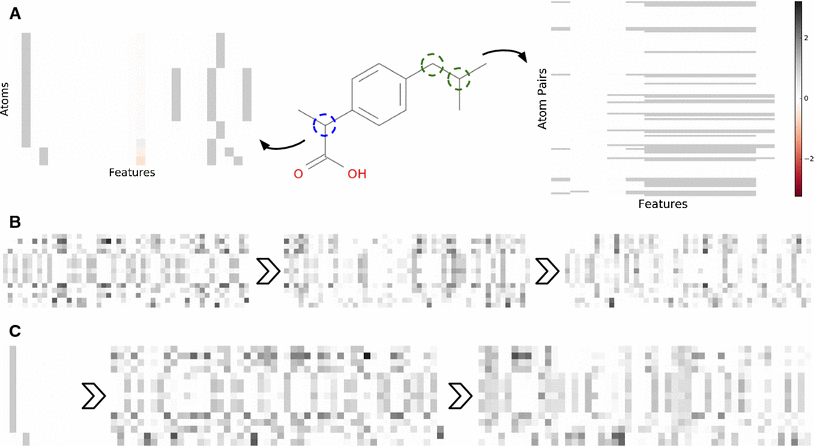
\includegraphics[width=.9\linewidth]{10822_2016_9938_Fig8_HTML.png}
\caption{\label{fig:orga0957c9}
Example of how a molecule is mapped to input features, and how the input features change as training epochs pass. Taken from \parencite{Kearnes2016}.}
\end{figure}

\subsection{Unsupervised Training of Neural Networks}
\label{sec:orgf6a20ef}

Prior applications of NNs to quantum chemistry primarily used supervised training, with the goal of predicting a molecular energy or property with increasing accuracy. The supervised training of NNs requires a separate quantum chemical calculation on each input for each target property, which is not tenable for databases sizes that represent meaningful chemical space (such as PubChem\cite{doi:10.1021/acs.jcim.7b00083}) or any high-level calculation methods (such as coupled cluster).

An original use of unsupervised learning is for ``pretraining'', where the bottom layers in a NN are trained to reproduce the inputs before switching to supervised learning. Currently, unsupervised pretraining is not commonly used within the image classification community due to the discovery of better weight initialization and structural choices for the network (ReLUs for the activations, convolutional rather than directly-connected layers), rendering it unnecessary. In the future, as the both the size of available training sets (here, chemical databases) and NN architectures grows, unsupervised pretraining may take a more prominent role.

Unsupervised training of NNs is not without precedent in quantum chemistry; generative adversarial networks (GANs) have been used to generate ``hallucinated'' (fake or imperfect) representations of methanol trimers, which are then fed into a fully-connected NN to predict the three-body energy\cite{doi:10.1063/1.4973380}. Although the error is \textasciitilde{}\(2\times\) that of the standard Coulomb matrix-based NN, this may be due to the use of more convolutional than fully-connected layers in the GAN.

Rather than use unsupervised learning for network pretraining, I will use the dimensionality reduction capability of a denoising autoencoder\cite{VincentPLarochelleH2008} with only fully-connected layers to generate features that will be identified using layer-wise relevance propagation. The rendered hallucinations from the GANs (depth maps or D-maps) also provide an interesting connection back to LRP for future work.

\section{Research Plan}
\label{sec:orgfe20067}

\subsection{Specific Aim \#1: Reproduction of Existing Literature Neural Networks}
\label{sec:org9dafa45}

\subsubsection{Introduction}
\label{sec:orge543d02}

The \uline{objective} is to reproduce trained neural networks from the literature in order to create the foundation of the machine learning pipeline to be developed within this proposal and to serve as a validation baseline for further predictions. The \uline{hypothesis} is that published quantum chemical neural networks are entirely reproducible by connecting free, open-source tools. To test this hypothesis, I will reproduce the ML pipeline and results from \parencite{2017arXiv170205532F}, specifically the isotropic static polarizability \(\bar{\alpha}\) and the zero-point vibrational energy \(E_{\text{ZPVE}}\). The \uline{expected outcome} is a fully-worked and documented reproduction of neural networks from the literature that can serve as the basis for future pipelines within the wider chemistry and machine learning communities.

\subsubsection{Research Design}
\label{sec:org6633990}

Unfortunately, the learned models for the results presented in \parencite{2017arXiv170205532F} are not available, only descriptions of the architectures. Recreating the literature models requires an implementation of the model architecture and input data in the proper format.

There are two neural network-based architectures described in \parencite{2017arXiv170205532F}: Graph Convolutions \cite{Kearnes2016} (GC) and Gated Graph Neural Networks \cite{2015arXiv151105493L} (GG). These NN architectures are used again as baselines in \parencite{2017arXiv170401212G}. Since the original GC implementation referenced in \parencite{2017arXiv170205532F} is \href{https://github.com/tkipf/gcn}{openly available}\cite{kipf2016semi}, I will use the GC-based architecture with modifications described in section E5 of \parencite{2017arXiv170205532F}. Details for the GC architecture input, called the Molecular Graph representation, are shown in tables 1 and 2 of \parencite{2017arXiv170205532F} and reproduced here.

\begin{table}[htbp]
\caption{\label{tab:orgbd4a0b0}
The Molecular Graph (MG) input representation: single atom features}
\centering
\begin{tabu}{|lp{10.25cm}l|}
Feature & Description & Size\\
\hline
Atom type & H, C, N, O, or F (one-hot) & 5\\
Chirality & R or S (one-hot or null) & 2\\
Formal charge & Integer electronic charge & 1\\
Partial charge & Calculated partial charge & 1\\
Ring sizes & For each ring size (3-8), the number of rings that include this atom & 6\\
Hybridization & sp, sp\(^2\), or sp\(^3\) (one-hot or null) & 3\\
Hydrogen bonding & Whether this atom is a hydrogen bond donor and/or acceptor (binary values) & 2\\
Aromaticity & Whether this atom is part of an aromatic system & 1\\
\hline
 &  & 21\\
\end{tabu}
\end{table}

\begin{table}[htbp]
\caption{\label{tab:org6c6378c}
The Molecular Graph (MG) input representation: atom pair features}
\centering
\begin{tabu}{|lp{10.25cm}l|}
Feature & Description & Size\\
\hline
Bond type & Single, double, triple, or aromatic (one-hot or null) & 4\\
Graph distance & For each distance (1-7), whether the shortest path between the atoms in the pair is less than or equal to that number of bonds (binary values) & 7\\
Same ring & Whether the atoms in the pair are in the same ring & 1\\
Spatial distance & The Euclidean distance between the two atoms & 1\\
\hline
 &  & 13\\
\end{tabu}
\end{table}

The QM9 dataset consists of 134K molecules \cite{Ramakrishnan:2014ij} containing up to 9 heavy atoms from the elements C, N, O, and F, with a maximum number of 29 atoms. The representation in tables \ref{tab:orgbd4a0b0} and \ref{tab:org6c6378c} will result in an input size of \(21\binom{x}{1} + 13\binom{x}{2}\) for a given number of atoms \(x\), leading to a total length of 5,887 for the maximum number of 29 atoms in QM9. Inputs are available as modified XYZ files from the Quantum Machine website under the \href{http://figshare.com/collections/Quantum\_chemistry\_structures\_and\_properties\_of\_134\_kilo\_molecules/978904}{QM9 Dataset} section\cite{Ramakrishnan:2014ij,doi:10.1021/ci300415d}, which will be transformed into the Molecular Graph (MG) representation using RDKit\cite{rdkit} with Gasteiger partial charges as in \parencite{Kearnes2016}. I will then modify the Graph Convolutions architecture from \parencite{Kearnes2016} as described in Section E5 of \parencite{2017arXiv170205532F}. Using the model parameters described in that section, I will train two separate models, one for the isotropic static polarizability \(\bar{\alpha}\), and another for the zero-point vibrational energy \(E_\text{ZPVE}\).

For the reproduction of literature results, the only numerical values from \parencite{2017arXiv170205532F} are in Table 3, which shows the mean absolute error (MAE) for each input representation-architecture combination. Because the sample size of QM9 is sufficiently large (134K molecules), the MAE is calculated using out-of-sample validation, where the ML models are trained using 90\% of the available data and compared against the DFT (B3LYP/6-31(2df,p)) results for the remaining 10\%. The 90\% constitutes \textasciitilde{}117K molecules after removing 3K from 134K due to failed SMILES consistency tests. This 90/10 (training + validation)/test set split allows for 10-fold cross-validation. It is not mentioned how the concrete splits are obtained or how the final MAE is calculated from the 10 models. For this proposal, I will perform an unbiased random shuffle of QM9 index codes and split them into 10 uniform bins. After training and model validation using the procedure described above, the final MAE will be calculated as the mean of the 10 individual MAEs. The literature models will be considered replicated if the two final models have MAEs within 95\% of 0.227 \(a_{0}^{3}\) for the polarizability and 0.00975 eV for the ZPVE, respectively.

\subsubsection{Expected Outcomes}
\label{sec:orgd37907b}

The concrete products of this aim will be a set of Python scripts that transform the XYZ-like files into the Molecular Graph representation, implement the modified Graph Convolutions architecture, train MG/GC models for each molecular property (\(\bar{\alpha}\) and \(E_\text{ZPVE}\)) using out-of-sample cross-validation, and calculate each molecular property from the trained models when given a normal XYZ molecular structure. This will be a fully-worked and documented reproduction of neural networks from the literature that can serve as the basis for not only this proposal's later aims, but for future pipelines within the wider chemistry and machine learning communities. These scripts will take the form of Jupyter Notebooks \cite{jupyter,PER-GRA:2007}, which combine code, math, and documentation in an easy-to-replicate package that is popular in the machine learning community.

\subsection{Specific Aim \#2: Characterization of Existing Literature Neural Networks}
\label{sec:org8b4f363}

\subsubsection{Introduction}
\label{sec:orgae04123}

The \uline{objective} is to quantify what already-published neural network-based ML models have learned. The \uline{hypothesis} is that when predicting an output, the most important (relevant) parts of the input for that output align with our trained chemical intuition. Specifically, for strongly geometry-dependent properties, such as the ZPVE, more relevance will be placed on geometric input features such as bond lengths and bond types. For strongly wavefunction- or density-dependent properties, such as the isotropic polarizability, more relevance will be placed on electronic input features such as partial atomic charges compared to other features. To test this hypothesis, I will develop the necessary ML pipeline for adding relevance propagation and analysis steps to the already-published ML models. This will involve connecting existing relevance propagation tools \cite{JMLR:v17:15-618,github:lrp,github:lrp_tf,github:lrp_tf2} to the end of the pipeline from aim \#1 and creating a human-understandable representation of the relevance propagation output in terms of molecular features.

\subsubsection{Research Design}
\label{sec:orgdc240db}

The authors of the relevance propagation algorithm I will use have created an open-source reference implementation in Python. From their GitHub page\cite{github:lrp}:

\begin{quote}
The Layer-wise Relevance Propagation (LRP) algorithm explains a classifier's prediction specific to a given data point by attributing relevance scores to important components of the input by using the topology of the learned model itself. The LRP Toolbox provides simple and accessible stand-along implementations of LRP for artificial neural networks supporting Matlab and Python.
\end{quote}

This reference implementation is interfaced with its own implementation of composable neural networks. This is not immediately compatible with the TensorFlow-based implementation of the Graph Convolutional neural networks trained in aim \#1. However, there is open-source initial interface code available for connecting TensorFlow-based models with LRP\cite{github:lrp_tf,github:lrp_tf2}. I will use these three implementations to write a Python interface between the trained GC models and LRP.

Once the LRP implementation is connected to the trained models, details of running the LRP algorithm must be considered. There are multiple decomposition variants of LRP, each with different trade-offs regarding numerical stability and conserving relevance\cite{Binder2016}. Because the number tunable parameters is small, with only one for each of the three variants, and there are examples of modulating these parameters in the literature, I will start with the variant that requires no free parameters and extend to the other variants if results do not make sense.

All examples from the relevance propagation literature focus on explaining image classification decisions using heat maps overlaid on the input image decision boundary. Instead of performing image classification, the neural networks trained in aim \#1 perform regression using a graph-type, heterogeneous input, so a different form of interpreting the results will be needed. LRP produces output on a per-sample basis with a signed relevance value for each input feature, where the sum of all relevance values equals the prediction output. For each molecule in the QM9 dataset, I will run the LRP implementation and perform the equivalent of feature normalization and scaling so that the relevances have zero mean with a minimum and maximum corresponding to the largest absolute values in the QM9 dataset. Not all molecules in QM9 have the same number of atoms, so for each molecule I will average together the relevances over all atoms to produce a single relevance for each type of feature (12 total). While this can be viewed as a significant loss of information, the goal of this proposal is to identify what types of features are generally important for different molecular properties, \uline{not} the quality of a prediction for a specific molecule.

\subsubsection{Expected Outcomes}
\label{sec:orga206b60}

Once LRP is applied to the trained models, \fxnote{TODO}

Additionally, the LRP analysis will be attached to the pipeline developed in aim \#1, with complete documentation and code that replicates the work from this proposal.

\subsection{Specific Aim \#3: Training Neural Networks for Complex Molecular Properties}
\label{sec:org13736cb}

\subsubsection{Introduction}
\label{sec:org39c39f0}

The \uline{objective} is to see how currently used neural network architectures perform for more complex molecular properties than those found in the literature. The \uline{hypothesis} is that the more complex properties \(\beta_{\parallel}\) and \(\{\tilde{\nu}\}\) are expected to have larger relative errors compared to \(\bar{\alpha}\) and \(E_{\text{ZPVE}}\), in particular the set of vibrational frequencies, as predictions of the highest fundamental frequency \(\omega_1\) alone already have large errors \cite{2017arXiv170205532F}. Testing this hypothesis first requires calculating the hyperpolarizability for each of the training samples, followed by training the network itself.

\subsubsection{Research Design}
\label{sec:org9a05db3}

Results for \(\{\tilde{\nu}\}\) are already present as labeled data in the QM9 dataset \cite{Ramakrishnan:2014ij}. I will use the \textsc{Dalton} quantum chemistry program package \cite{daltonpaper} for the hyperpolarizability calculations, as it is free for academic use and designed especially for the calculation of molecular response properties such as hyperpolarizabilities. These calculations will employ the B3LYP density functional in combination with the 6-31G(2df,p) basis set to maintain comparability with past calculations from the QM9 dataset \cite{Ramakrishnan:2014ij}.

Training the NN-based model for the hyperpolarizability will not require any modifications to the NN architecture, as \(\beta_{\parallel}\) is a scalar quantity. As the set of vibrational modes is dependent on molecular size, the architecture that will be trained to reproduce \(\{\tilde{\nu}\}\) will be modified to output the maximum possible number of vibrational frequencies, with the first \(3N-6\) output nodes returning predictions and the remainder padded with zeros. This is a well-known limitation of many ML architectures using variable-dimension input and output.

The error metric used for the set of vibrational frequencies will be identical to that for \(\omega_1\), which has an MAE of 3.15 cm\(^{-1}\). The error in harmonic vibrational frequencies is not uniformly distributed among all normal modes\fxnote{[REF]}, but comparing the literature error for \(\omega_1\) against the same value trained on a network for all vibrational frequencies is a measure of how a joint NN compares to a separate NN for each vibrational frequency. For the hyperpolarizability, the MAD of the DFT calculations used in training will be used as the baseline for the MAE of the trained NN prediction. In both cases, since training is occurring on novel properties rather than replicating literature values, achieving DFT accuracy is the goal for training convergence.

\subsubsection{Expected Outcomes}
\label{sec:orgfd391f5}

Similar to aim \#1, the result will be a full set of documented Jupyter Notebooks that parse the hyperpolarizability calculation outputs and train separate MG/GC models for the hyperpolarizability and vibrational frequencies. In addition to the trained models, I will provide the raw calculation outputs for the hyperpolarizability calculations on figshare\cite{figshare}, which is capable of hosting large archives. These outputs will contain full dipole, polarizability, and hyperpolarizability tensors, along with other common quantities from quantum chemical calculations such as L$\backslash$``owdin partial atomic charges and MO coefficients. Distributing these unmodified outputs enables the future prediction of even more complex properties

\subsection{Specific Aim \#4: Characterization of Novel Neural Networks}
\label{sec:orgc22961e}

\subsubsection{Introduction}
\label{sec:org3a318ab}

The \uline{objective} is to determine the relative importance of each component in the molecular representation to predictions of complex molecular properties. The \uline{hypothesis} is that the most important input features for \(\beta_{\parallel}\) and \(\{\tilde{\nu}\}\) are similar to those for \(\bar{\alpha}\) and \(E_{\text{ZPVE}}\), respectively. This will be done by applying the analysis techniques developed in aim \#2 to the neural networks trained in aim \#3, along with

\subsubsection{Research Design}
\label{sec:org02bf692}

\begin{anfxnote}{nn construction}
The basic structure of the unsupervised network will be as follows. It will be a denoising autoencoder (DAE) with an input layer of the same dimension as the GC input, a coding layer of dimension ???, and a hidden layer between the input and coding layers. This will be a symmetric structure where the weights of the encoding and decoding sections are tied, meaning they are constrained to be identical. I will adapt the Molecular Graph input from aim 1 on top of this denoising autoencoder as implemented in TensorFlow\cite{tensorflow2015-whitepaper,github:tf,github:tf_dae}. Because a DAE reconstructs its inputs and does not make a classification or regression prediction, only one model needs to be trained, not four. Here I should describe how the DAE will be trained? How to decide on dimension of intermediate and coding layers? Once the DAE model is trained, it will replace the input layer for each of the trained supervised networks. If the DAE is capable of performing good input reconstruction, then the prediction performance of these combined networks should not be much worse than the supervised networks for the training, but may be improved on validation and testing.

Performance may decrease because the reconstruction of the original input cannot be perfect, which would constitute overfitting.

Some of this can go in aim 4!

Could LRP be performed on the DAE itself? Could be another test of quality for the input reconstruction

The purpose of adding the autoencoder structure is that using layer-wise relevance propagation will show the relevance of the \emph{encoded} input. The expectation is that because the learned encoding retains only important features for the input, xxx rather than using the possibly overcomplete input feature description. If the DAE is good at reconstructing the inputs

The original purposes of generative pretraining are to prevent overfitting in large neural networks and learn structure in large amounts of unlabeled data.

Larger databases already exist \cite{doi:10.1021/acs.jcim.7b00083}

In the future, with larger amount of unlabeled data (we don't want to have to run millions of hyperpolarizability calculations in order to train), such as in \parencite{doi:10.1021/acs.jcim.7b00083},

In the future, it may make sense to unfreeze the autoencoder weights and change them slightly via backpropagation, so the autoencoder learns a redudced-dimensionality encoding that is more optimal for the network output and not just reconstructing the input.
\end{anfxnote}

\subsubsection{Expected Outcomes}
\label{sec:orgff5dc86}

\begin{itemize}
\item Models with unsupervised learning steps have improved prediction accuracy of chemical properties compared to those without. \fxnote{That is, the models developed and trained in this aim should show better prediction performance than the literature models from aim \#1. This implies the models from this aim are of higher-quality and are more likely to have "learned correctly" in the sense that they learned "chemical intutition".}

\item The parameters learned by ML models, and therefore their predictions, will show a strong dependence on the input features in chemically-intuitive manner.
\item Neural network-based ML architectures are a valid path forward for predicting novel and more complex chemical properties.
\end{itemize}

\section{Broader Impacts}
\label{sec:orgbc5f4aa}

A crucial reason for the growth in cross-disciplinary applications of machine learning is the openness and extensiveness of introductory tools, specifically tutorials and examples. Historically, chemistry lags behind other sciences in terms of openness of procedures and results. The current infrastructure surrounding the combination of machine learning and quantum chemistry is very poor: disorganized work, disorganized results, and not all components are available for reuse. The development of these machine learning pipelines will constitute the development of open-source, freely available infrastructure that will be easily extendable. \uline{I will provide openly \textbf{all} components of the machine learning pipeline developed in this proposed work}, including the fully-trained models, meaning the implementations using open-source software and the learned parameters for each model. All components will be placed on \href{https://github.com/}{GitHub}, the premier location for the open hosting of machine learning tools. Making these tools available will enable the verification of future, more advanced machine learning models that has not been possible to date. The tools will also serve as a pedagogical example for how machine learning can be applied to quantum chemical problems.

As the application of machine learning within quantum chemistry is relatively new and fast-moving, still being in the ``discovery'' phase, there have not been attempts at replicating machine learning pipelines, peer-reviewed or otherwise. Additionally, in traditional quantum chemistry there are a plethora of well-known program packages for performing electronic structure calculations \cite{g16,QCHEM4,daltonpaper,WCMS:WCMS93} that are self-contained, \emph{e.g.} a single program can calculate optimized geometries, vibrational spectra, NMR chemical shifts, reaction energies, etc. This infrastructure exists to some degree for machine learning, with base packages such as scikit-learn \cite{scikit-learn} and TensorFlow \cite{tensorflow2015-whitepaper} themselves being self-contained with excellent tutorials and examples, however this infrastructure does not exist for quantum chemistry-derived machine learning models. Introductions to machine learning are numerous and extensive using the standard ``fruit fly'' of NNs, the MNIST database of handwritten digits \cite{lecun-01a}, and similar fully-worked introductions should exist for quantum chemistry as well. Releasing the pipeline from this proposal allows it to serve as the ``fruit fly'' for quantum chemistry in machine learning.

\printbibliography
\listoffixmes
\end{document}
